\documentclass[a4paper,10pt]{article}
\usepackage{amsmath}
\usepackage{graphics}
\usepackage{graphicx}
\usepackage{listings}
\usepackage[svgnames]{xcolor}
\begin{document}
	
\title{User Manual for \textbf{int\_spline}}
\author{Yuriy Korablev}

\maketitle

\lstset{ %
	language=R,                   
	basicstyle=\small\sffamily,   
	%numbers=left,                
	%numberstyle=\tiny,          
	%stepnumber=1,                  
	%numbersep=5pt,                
	backgroundcolor=\color{white}, 
	showspaces=false,            
	showstringspaces=false,      
	showtabs=false,             
	%frame=single,              
	tabsize=2,                
	captionpos=t,              
	breaklines=true,           
	breakatwhitespace=false, 
	%escapeinside={\%*}{*)},   
	keywordstyle=\color{blue},
	keywords={NULL,FALSE,TRUE,if, INF, for, while, break,else,return,library,function},%
	otherkeywords={!,!=,~,\$,\&,\%/\%, \%*\%,\%,^,<-,<<-},
	%alsoother={._\$},
	sensitive,%
	morecomment=[l][\color{lightgray}\itshape]\#,%
	morestring=[d]",%
	morestring=[d]'%
}

\section{Installation}
Copy and open the script file \lstinline|"int_spline example.R"| or implement the below code. 
As data files, copy \lstinline|"fig1.csv"|, \lstinline|"fig3.csv"| or \lstinline|"purchases.csv"| files.

\section{Implementation}
Function \textbf{int\_spline} has following arguments:
\begin{itemize}
	\item \lstinline|t| - array of $n$ observation coordinates $t_i$;
	\item \lstinline|Y| - array of $n-1$ observation values $y_i$;
	\item \lstinline|s| - array of knots $s_k$, by default the same as t;
	\item \lstinline|m| - number of knots, by default \lstinline|length(s)|;
	\item \lstinline|W| - array of weights $w_i$, by default vector of 1;
	\item \lstinline|alpha| - smoothing parameter, by default $10^5$;
	\item \lstinline|x| - array of coordinates in which the spline values will be calculated and returned; by default, it ranges from $t_1$ to $t_n$ with a step size of 1;
	\item \lstinline|info| - indicator of whether to return additional information or not, by default FALSE.
\end{itemize}

In a case where number of knots \lstinline|m| is defined, but knots \lstinline|s| itself are not defined, knots \lstinline|s| are calculated as equally spaced (function \lstinline|seq| return sequence between $t_1$ and $t_n$).
%
\begin{lstlisting}[language=R]
	n=length(t)
	if (m!=length(s)) 
		s=seq(t[1],t[n],length=m)
\end{lstlisting}
%
Whenever knots \lstinline|s| was defined or calculated, the distance between knots $h_k=s_{k+1}-s_k$ is calculated.
%
\begin{lstlisting}[language=R]   
	h=array(0,dim=m-1)
	h[1:(m-1)]=s[2:m]-s[1:(m-1)]
\end{lstlisting}
%
Filling in matrices $Q$ and $R$. 
Note, that in main article (subsection 2.1) we depicted column's number starting from 2, but here we start indexing columns from 1 (i.e. element $Q[1,1]$ here is element $Q[1,2]$ from section 2.1).
Same for row's number in matrix $R$, they should start from 2, but here we start from 1 (i.e. element $R[1,1]$ here is element $R[2,2]$ from section 2.1).
%
\begin{lstlisting}[language=R]
	Q=matrix(0,nrow=m,ncol=m-2)
	for (i in 1:(m-2))
	{
		Q[i,i]=1/h[i]
		Q[i+1,i]=-1/h[i]-1/h[i+1]
		Q[i+2,i]=1/h[i+1]
	}	

	R=matrix(0,nrow=m-2,ncol=m-2)
	for (i in 1:(m-2))
	{
		R[i,i]=1/3*(h[i]+h[i+1])
		if (i<m-2)
		{
			R[i+1,i]=1/6*h[i+1]
			R[i,i+1]=1/6*h[i+1]
		}
	}	
\end{lstlisting}
%
After that we calculate matrix $K=QR^{-1}Q^T$, but some intermediate calculations ($R^{-1}$ and $Q^T$) will repeat later, so its better to save them in the corresponding variables (here function $solve(R)$ returns inverse matrix, $t(Q)$ returns transposed matrix and operation \lstinline|%*%| denote matrix multiplication).
%
\begin{lstlisting}[language=R]
	inv_R=solve(R)  
	t_Q=t(Q)
	K=Q %*% inv_R %*% t_Q
\end{lstlisting} 
%
The hardest part is filling in $V$ and $P$ matrices depending on how the observations landed on the knots intervals. 
For each row $i$ we need to find on which $k$-th interval the $i$-th observation has landed and in how many intervals $L$ the $i+1$-th observation has landed \footnote{Remark. If we have integrals $y_i$ defined on arbitrary intervals $[t_a[i],t_b[i]]$, which may even intersect, all that needs to be changed here is to use $t_a[i]$ instead of $t[i]$, $t_b[i]$ instead of $t[i+1]$ and define $k$ inside the loop. }.
Note, that for correct indexing we are filling in the matrix $P$ as if it had $m$ columns, and later we discard the first and last column. 
%
\begin{lstlisting}[language=R]
	V=matrix(0,nrow=n-1,ncol=m)
	P=matrix(0,nrow=n-1,ncol=m)
	k=1
	while( (s[k]<=t[1]) & (s[k+1]<t[1])) #find k, that s[k+1]>t[1]
		k=k+1
	for (i in 1:(n-1))
	{
		#finding L, it can be 0
		for (L in 0:(m-k-1))
			if (t[i+1]<=s[k+L+1])
				break
		l=1;
		V[i,k]=(s[k+1]-t[i])^2/h[k]/2  
		P[i,k]=h[k]^3/24-(t[i]-s[k])^2*(s[k+1]-t[i]+h[k])^2/h[k]/24 
		while (l<=L)
		{
			V[i,k+l]=(h[k+l-1]+h[k+l])/2
			P[i,k+l]=(h[k+l-1]^3+h[k+l]^3)/24
			l=l+1;
		}
		V[i,k+1]=V[i,k+1]-(t[i]-s[k])^2/h[k]/2
		P[i,k+1]=P[i,k+1]+(t[i]-s[k])^2
			*((t[i]-s[k])^2-2*h[k]^2)/h[k]/24
		V[i,k+L]=V[i,k+L]-(s[k+L+1]-t[i+1])^2/h[k+L]/2
		P[i,k+L]=P[i,k+L]+(s[k+L+1]-t[i+1])^2
			*((s[k+L+1]-t[i+1])^2-2*h[k+L]^2)/h[k+L]/24    
		V[i,k+L+1]=(t[i+1]-s[k+L])^2/h[k+L]/2
		P[i,k+L+1]=h[k+L]^3/24-(s[k+L+1]-t[i+1])^2
			*(t[i+1]-s[k+L]+h[k+L])^2/h[k+L]/24
		k=k+L
	}
	P=P[1:(n-1),2:(m-1)] #don't need first and last column
\end{lstlisting}
%
Next we calculate the matrix $C=V-PR^{-1}Q^T$ and use the previously calculated matrices $R^{-1}$ and $Q^T$ for this.
%
\begin{lstlisting}[language=R]
	C=V-P %*% inv_R %*% t_Q
\end{lstlisting} 
%
Finally we calculate vector $g=\left(C^TWC+\alpha K\right)^{-1}C^TWY$ (spline values) and vector $\gamma=R^{-1}Q^Tg$ (second derivatives). 
Because matrix $C^T$ is used few times, we remember it to corresponding variable.
%
\begin{lstlisting} [language=R]
	t_C=t(C)
	W=diag(W)            # make matrix from vector of weights
	A=t_C %*% W %*% C + alpha * K
	g=solve(A , t_C %*% W %*% Y )
	gamma=inv_R %*% t_Q %*% g
\end{lstlisting} 
%
At this point, we have everything to build our spline (the spline is completely defined by means of $g$ and $\gamma$).
We calculate the spline values at arbitrary points $x$ (array), which are specified by the user and passed as an argument to our function \textbf{int\_spline} (if argument $x$ is omitted, then points are calculated as range from $t_1$ to $t_n$ with a step size of 1).
As result, values $y=g(x)$ (vector), $x$, $g$ and $\gamma$ are returned as a list.


%
\begin{lstlisting}[language=R]
	g2=c(0,gamma,0) #Second derivative on the edges was zero
	y=rep(0,length(x)) #x=seq(t[1],t[n],1) by default
	k=1; #index of interval 
	for (j in (1:length(x)))
	{
		while (x[j]<t[n] & x[j]>s[k]+h[k])
		k=k+1;
		y[j] = ((x[j]-s[k])*g[k+1]+(s[k+1]-x[j])*g[k])/h[k] 
		- 1/6*(x[j]-s[k])*(s[k+1]-x[j])*(g2[k+1]*(1+(x[j]-s[k])/h[k])
		+g2[k]*(1+(s[k+1]-x[j])/h[k]))
	}
	if (info)
	{
		result=list(x=x,y=y,g=g,gamma=g2,s=s,h=h)
		return (result)
	}
	else 
		return(y)
\end{lstlisting} 


\section{Application} \label{sec:application}
Data input. Assume the data set represented in the \lstinline|.csv| file, which has two columns: Date and Value. Data from this \lstinline|.csv| file can be input using the following lines of code:
%
\begin{lstlisting}[language=R]
	library(lubridate)
	filename="F:/FilePath/FileName.csv";
	
	#if CSV file was generated by Excel
	MyData = read.csv(file=filename, header=TRUE, sep=";",
		stringsAsFactors = FALSE, dec=",")
	t=as.numeric(dmy(MyData[[1]]))
	
	#if CSV file was generated by R
	#MyData = read.csv(file=filename, header=TRUE, sep=",",
		stringsAsFactors = FALSE, dec=".")
	#t=as.numeric(ymd(MyData[[1]]))
	
	t=t[!is.na(t)]
	n=length(t)
	Y=MyData[[2]]
	Y=Y[1:(n-1)] # Last value not used 
\end{lstlisting}
%
The simplest call to the proposed function, which calculates the spline, can be done with the following lines of code:
%
\begin{lstlisting}[language=R]
	r=int_spline(t,Y)	
	y=r$y
\end{lstlisting}
%
This function call causes the function to compute the spline defined by the knots, which coincide with observation dates. By default, spline values are calculated at every point between the first and last observations (the x-coordinates are not returned by default; \lstinline|x=t[1]:t[n]| must be defined before plotting the graph). 
\\
Plotting the spline with a graph of average values using the following code lines
%
\begin{lstlisting}[language=R] 
	x2=NULL    #graph of average values
	y2=NULL
	for (i in 1:(n-1))        
	{
		x2=c(x2,t[i],t[i+1])
		y2=c(y2,Y[i]/(t[i+1]-t[i]),Y[i]/(t[i+1]-t[i]))
	}
	
	plot(x,y,col="red",type="l",lwd="1",lty=1, xaxt="n",
	ylim=range(c(y,y2)),xlim=range(c(x,x2)))
	axis.Date(1, at=seq(min(dmy(MyData[[1]])),
	max(dmy(MyData[[1]])), by="months"),
	format="%m-%Y")
	lines(x2,y2,col="black",type="l",lwd="2",lty=1)
	
\end{lstlisting}
%
As a result, the function has been restored by integrals, as shown in Figure~\ref{fig:coincide_observations}.
The algorithm clearly tries to fit a spline so that the area under the function tends to the area under each step (with the roughness penalty).
%
\begin{figure}[h]
	\centering
	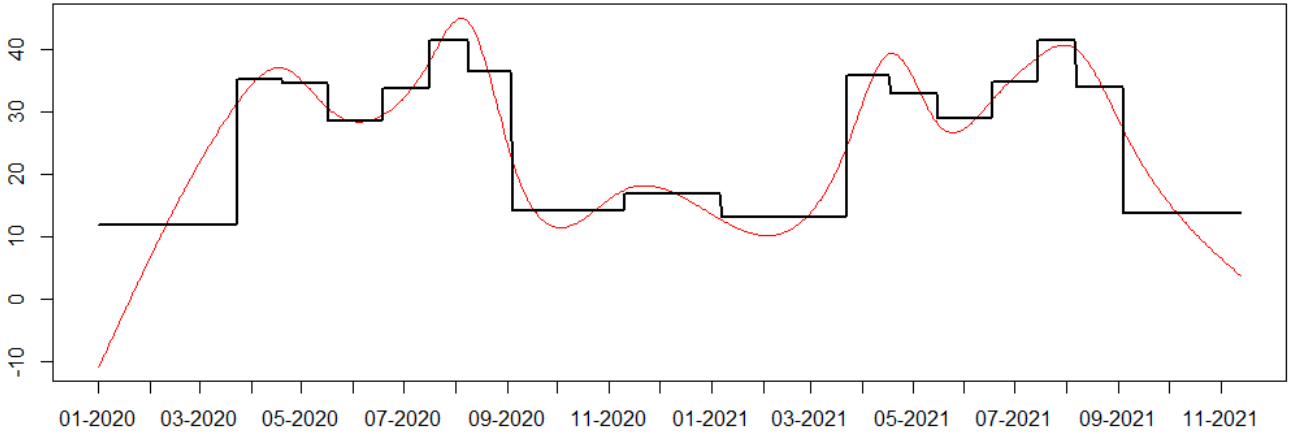
\includegraphics[width=\linewidth]{coincide_observations.png}
	\caption{\label{fig:coincide_observations} Restored function, simplest call.}
	% \Description{} not working
	\small{ Staircase line shows the average values $y_i/(t_{i+1}-t_i)$. The area under each stair step represents the observed integral $y_i$.}
\end{figure}
%
%
Figure~\ref{fig:coincide_observations} also shows that the distance between observations (and knots) varies. This creates a strange incline in the restored function.
If knots had been chosen in another way (equally spaced), the graph would be different.
For example, with the same number of knots $n$, but spaced equally, the result is as shown in Figure~\ref{fig:equally_spaced} with the  following code lines:
\begin{lstlisting}[language=R]
	s=seq(t[1],t[n],length=n)
	y=int_spline(t,Y,s=s)	
\end{lstlisting}
%
\begin{figure}[h]
	\centering
	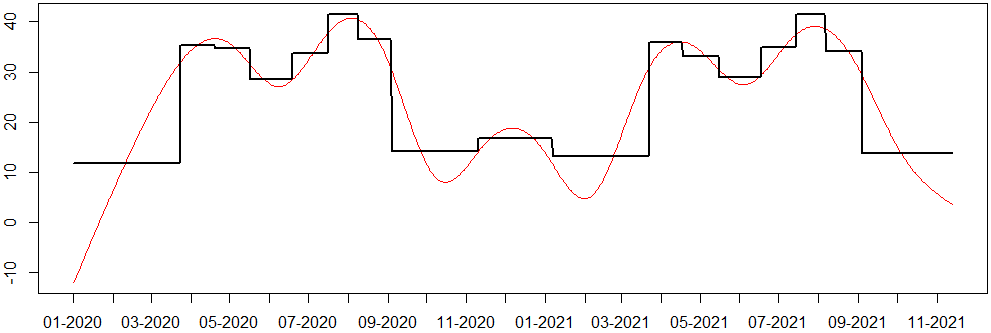
\includegraphics[width=\linewidth]{equally_spaced.png}
	\caption{\label{fig:equally_spaced}  Restored function, equally spaced knots.}
\end{figure}

It is not necessary to define the knot sequence \lstinline|s| every time, it is enough to define the number of knots \lstinline|m|.
The number of knots \lstinline|m| can be less than or greater than the number of observations \lstinline|n|.
Without a knot sequence \lstinline|s| defined, if \lstinline|m| is defined as not equal to \lstinline|n|, the resulting knot sequence will be equally spaced (if \lstinline|m| is defined equal to \lstinline|n|, the knots will coincide with the observation points).
For example, a simple function call to calculate a spline with equally spaced knots could be the following:
\begin{lstlisting}[language=R]
	y=int_spline(t,Y,m=n*3)	
\end{lstlisting}
The number of knots \lstinline|m| does not have much influence on the resulting curve until it is more than two times less than \lstinline|n|.
The greatest effect is exerted by the smoothing parameter $\alpha$ (by default $\alpha=10^5$, and the second derivative is much less than the integrals).
If $\alpha$ is zero, then no smoothing takes place.
If $\alpha$ is too large (for example, $10^{10}$ or greater), the function tends to a straight line. 
However, for some data sets, the parameter $\alpha$ has almost no effect until it becomes large enough to start straightening the restored function.
For example, for the same data set that was used to generate Figure~\ref{fig:coincide_observations}), $\alpha$ had no visible effect from 0 to $10^4$.
This happened because there was little noise in the data and the spline was computed in an almost perfect way.
Any deviation from the resulting shape will cause significant errors (with the roughness penalty much weaker that these errors).
For noisy data, large errors are already present, and any slight change in the roughness penalty will lead to changes in spline shape.
For example, for another data set, changing the smoothing parameter $\alpha$ from $\alpha=10^5$ to $\alpha=10^4$ had a strong influence on the resulting graphs.
In Figure~\ref{fig:smoothing_parameter}a and Figure~\ref{fig:smoothing_parameter}b, note that the restored function shows strange behavior on the second peak.
\begin{figure}[h]
	\centering
	\begin{minipage}[h]{0.49\linewidth}
		\center{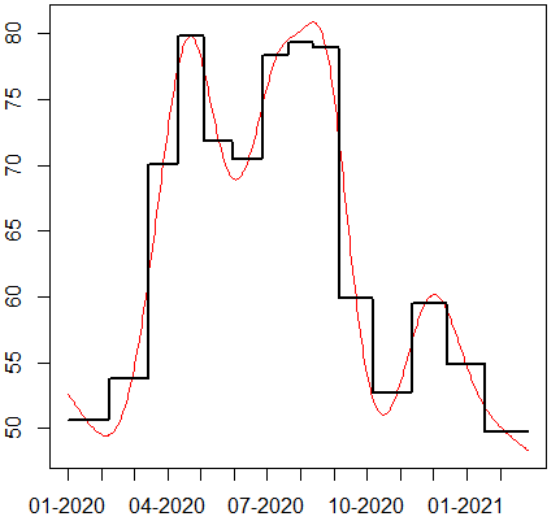
\includegraphics[width=0.9\linewidth]{a_10_5.png} \\ a)}
	\end{minipage}
	\hfill
	\begin{minipage}[h]{0.49\linewidth}
		\center{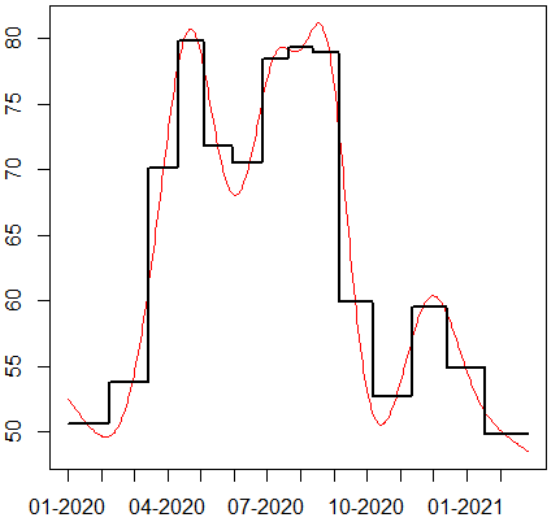
\includegraphics[width=0.9\linewidth]{a_10_4.png} \\ b)}
	\end{minipage}
	\caption{\label{fig:smoothing_parameter}  Restored by integrals function with a) $\alpha=10^5$ and b) $\alpha=10^4$}
\end{figure}

It is also possible to define weights for individual observations.
A weight of 0 will make the algorithm ignore the associated observation, whereas a weight greater than 1 will make the algorithm pay more attention to the associated observation.
For example, to improve spline shapes in Figures~\ref{fig:smoothing_parameter}a and b, one can place a weight of 0 on the 8-th observation and a weight of 100 on the 4-th observation using the following code lines: 

\begin{lstlisting}[language=R]
	W=rep(1,n-1)
	W[8]=0
	W[4]=100
	y=int_spline(t,Y,m=n*3,alpha=10^4,W=W)
\end{lstlisting} 

As a result, in Figure~\ref{fig:with_weights}, the depression on the second peak has disappeared, and the peak on the fourth observation has become slightly higher.
With these changes, it is difficult to see any difference between the two graphs. 

\begin{figure}[h]
	\centering
	\begin{minipage}[h]{0.49\linewidth}
		\center{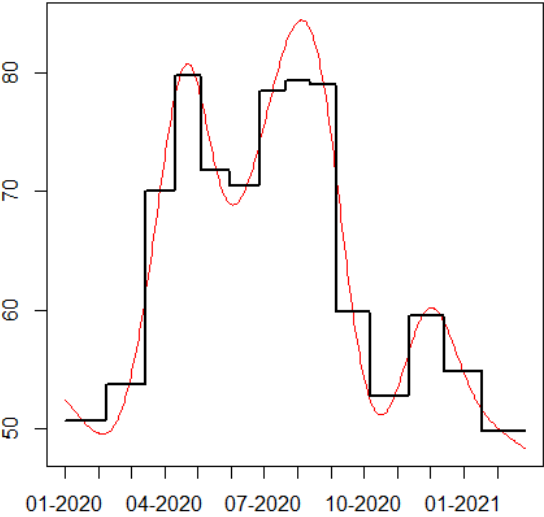
\includegraphics[width=0.9\linewidth]{weights_a_10_5.png} \\ a)}
	\end{minipage}
	\hfill
	\begin{minipage}[h]{0.49\linewidth}
		\center{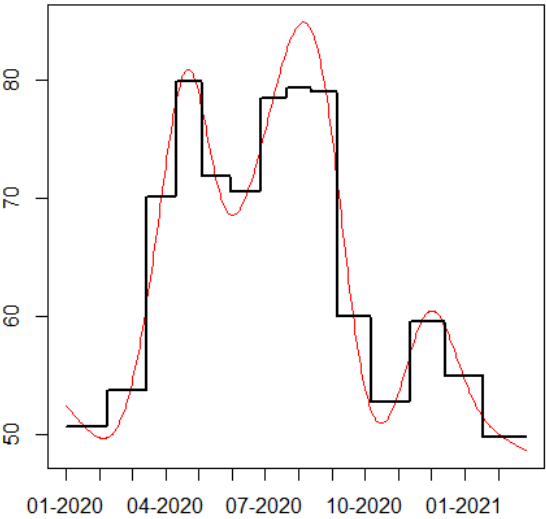
\includegraphics[width=0.9\linewidth]{weights_a_10_4.png} \\ b)}
	\end{minipage}
	\caption{\label{fig:with_weights} Same as Figure \ref{fig:smoothing_parameter} but with weights $w_4=100, w_8=0$, a) $\alpha=10^5$ and b) $\alpha=10^4$}
\end{figure}

As mentioned earlier, by default, spline values are calculated at every point between the first and last observations.
To calculate a spline at other points, it is only necessary to define the vector \lstinline|x|.
By the following lines to calculate the spline at every 15th point, the result is as shown in Figure~\ref{fig:every_15th}: 
\begin{lstlisting}[language=R]
	x=seq(t[1],t[n],15)
	y=int_spline(t,Y,m=n*3 ,alpha=10^5,x=x)	
\end{lstlisting}
\begin{figure}[h]
	\centering
	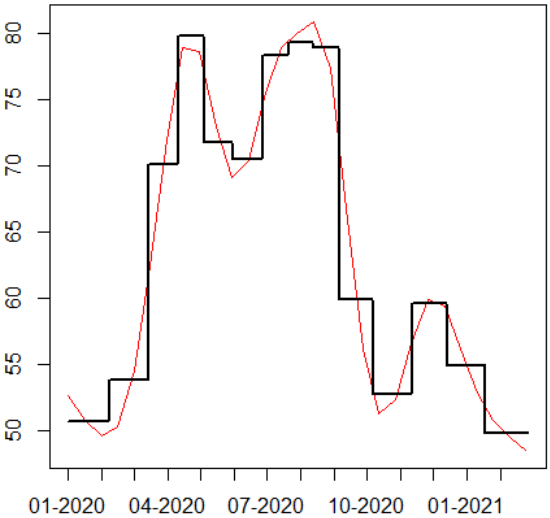
\includegraphics[width=0.49\linewidth]{every_15th.png}
	\caption{\label{fig:every_15th}  Calculating spline at every 15 points.}
\end{figure}

\end{document}